\documentclass[conference]{IEEEtran}
\usepackage[utf8]{inputenc}
\usepackage[spanish,es-tabla,es-nodecimaldot]{babel}
\usepackage{amsmath,amssymb}
\usepackage{graphicx}
\usepackage{booktabs}
\usepackage{url}
\usepackage{microtype}
\usepackage{hyperref}
\hypersetup{colorlinks=true,linkcolor=black,citecolor=blue,urlcolor=blue}
\graphicspath{{../resultados/figuras/}}
\newcommand{\Lh}{\hat L}

\title{Tarea 2: Tópicos en Grandes Volúmenes de Datos\\
Sketch de Cauchy para estimar cuánto cambia el tráfico de una red}
% TODO: confirmar integrantes del grupo
\author{Diego Pérez, Antonia Montero y Angie Ramirez\\
Repositorio: \url{https://github.com/Diego-ipt/GVdD_T2}}

\begin{document}
\maketitle

\section{Implementación (Actividad 1)}

\textbf{Lenguaje y estructura.} C++17 (g++~13.3, \texttt{-O2 -march=native}) para el sketch, la caché y la referencia exacta; Python~3.12 (numpy, pandas, matplotlib) para tablas y figuras. Las trazas MAWI (samplepoint-F, 25, 26 y 30 de enero de 2018, 14:00~h) se convirtieron con \texttt{pcap2bin} de la Tarea~1: se obtienen $103{,}7$, $102{,}2$ y $93{,}2$~M paquetes IPv4 (se descartan $4{,}1$, $4{,}3$ y $2{,}5$~M IPv6), sin paquetes fuera de orden. La clave es siempre la IP de destino. \texttt{reproducir.sh} corre todo sin intervención manual.

\textbf{Sketch.} \texttt{src/cauchy.hpp} implementa el Algoritmo~1 literalmente: \textsc{Mezclar} es splitmix64 y $C_{ji}=\tan(\pi(u-\frac12))$ con $u=(\lfloor h/2^{12}\rfloor+\frac12)2^{-52}$ y $h=\textsc{Mezclar}(g_j\oplus i)$. La única aceleración es precalcular las $k$ semillas de fila $g_j=\textsc{Mezclar}(\textsc{Mezclar}(\sigma)\oplus j)$. \textsc{EstimarDistancia} exige el mismo $k$ y la misma $\sigma$ y toma la mediana con \texttt{nth\_element}. Como \textsc{Entrada} no depende de $k$, una sola corrida con $k=512$ entrega también $k=32$ y $k=128$ (prefijos), y todos los $T$ se procesan en una pasada, cada uno con sus sketches $A,P$ y su caché.

\textbf{Diseño de la caché.} Es una caché de \emph{mapeo directo} de $B$ ranuras $(ip,c)$ ($8B$ bytes). La IP $i$ solo puede ocupar la ranura $h(i)=\lfloor \mathrm{fmix32}(i)\,B/2^{32}\rfloor$, y $c=0$ indica una ranura vacía:
\begin{itemize}
\item \textsc{Registrar}$(S,K,i)$: $r\gets h(i)$. Si $K[r]=(i,c)$ con $c>0$, se hace $c\gets c+1$. Si no, cuando $K[r].c>0$ se llama \textsc{Actualizar}$(S,K[r].ip,K[r].c)$ (expulsión), y luego $K[r]\gets(i,1)$. Costo O(1) en el peor caso.
\item \textsc{Vaciar}$(S,K)$: para cada $r$ con $K[r].c>0$, se llama \textsc{Actualizar}$(S,K[r].ip,K[r].c)$ y se hace $K[r].c\gets 0$. Costo $O(B)$ más las llamadas.
\end{itemize}
\emph{Invariante:} $S.y = C\,(x^{\mathrm{reg}}-x^{K})$, donde $x^{\mathrm{reg}}$ son las cuentas de los paquetes registrados y $x^K$ el contenido de la caché. Es decir, cada paquete está en el sketch o en la caché, nunca en ambos ni en ninguno. \emph{Exactitud:} el invariante vale al inicio (todo es 0). Un acierto o una inserción en una ranura vacía suben $x^{\mathrm{reg}}_i$ y $x^K_i$ en 1. Una expulsión suma $c'C_{\cdot,i'}$ a $S.y$ y baja $x^K_{i'}$ en $c'$. \textsc{Vaciar} hace lo mismo con cada ranura y deja $x^K=0$. Por lo tanto, tras \textsc{Vaciar}, $S.y=Cx^{\mathrm{reg}}$: lo mismo que \textsc{Actualizar}$(S,i,1)$ por paquete, salvo el redondeo. $B$ se elige con \texttt{--B}, y en los experimentos se usó $B=4096$ (32~KiB).

\textbf{Verificación} (\texttt{bin/verify}). (i) Coinciden los valores de referencia del enunciado: \textsc{Mezclar}$(0)$\,=\,\texttt{0xE220A8397B1DCDAF} y \textsc{Entrada}$(42,j,192.168.0.1)=-0{,}889927650$; $-2{,}088573016$; $-26{,}926917514$. (ii) Sobre $2{,}5\cdot10^6$ entradas, la mediana de $|C_{ji}|$ es $0{,}9986$, y todos los cuantiles de $|C|$ entre 0,05 y 0,999 coinciden con $\tan(\pi p/2)$ (Fig.~\ref{fig:pesos}). (iii) $10^5$ triples $(\sigma,j,i)$ reevaluados en otro orden dan el mismo valor bit a bit, y el sketch de 1000 IPs en orden directo e inverso difiere en $1{,}5\cdot10^{-13}$. (iv) Una IP con cuenta $c\in\{1,10,10^3,10^6\}$ contra un sketch vacío (50 semillas) da $\Lh/c$ con media $1{,}040/1{,}005/0{,}990$ y desviación $0{,}296/0{,}136/0{,}065$ para $k=32/128/512$, frente a $0{,}278/0{,}139/0{,}069$ teóricos. (v) Caché: en los intervalos 1--2 del día~26 con $T=10$~s ($2{,}42$~M paquetes), $\Lh$ con $B=4096$ y $\Lh$ llamando a \textsc{Actualizar} por paquete difieren en $3{,}9\cdot10^{-12}$, $3{,}6\cdot10^{-12}$ y $2{,}9\cdot10^{-13}$ (relativo) para $k=32,128,512$. Una prueba sintética con $B=7$ ($\phi=0{,}99$, casi todo expulsiones) difiere en $10^{-15}$.

\textbf{Referencia exacta} (\texttt{bin/exact\_intervals}). Usa una tabla \texttt{unordered\_map<uint32,uint64>} por intervalo, con la misma regla de intervalos que el Algoritmo~2. Calcula $N_q$ y $L_q=\sum_i|x_{q,i}-x_{q-1,i}|$ recorriendo ambas tablas, y en modo \texttt{cross} compara dos trazas por intervalo y completas, y caracteriza las IPs que más aportan a $L$. Los $N_q$ del sketch y de la referencia coinciden en todos los intervalos, y \texttt{analisis.py} lo verifica.

\begin{figure}[t]
\centering
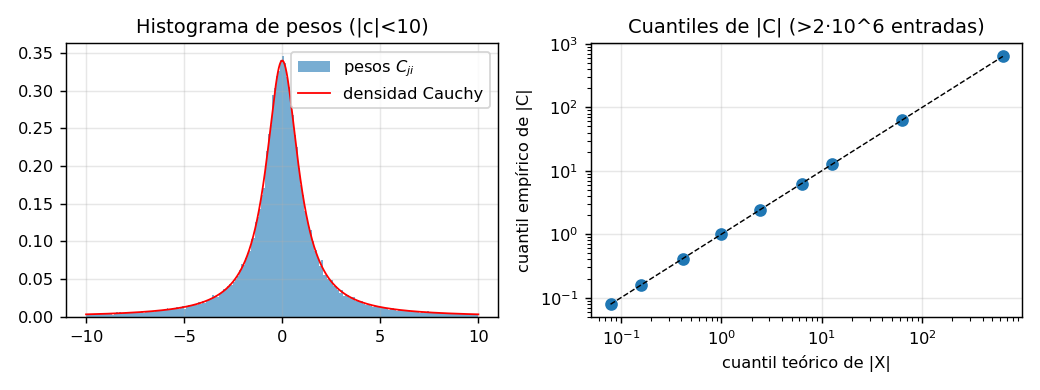
\includegraphics[width=\columnwidth]{verif_pesos.png}
\caption{Pesos $C_{ji}$: histograma frente a la densidad de Cauchy, y cuantiles empíricos de $|C|$ frente a los teóricos.}
\label{fig:pesos}
\end{figure}

\section{Intervalos consecutivos (Actividad 2.1)}

Se usó la traza del día 26 con $T\in\{10,30,60,120\}$~s, $k\in\{32,128,512\}$ y $\sigma\in\{1,\dots,5\}$. La duración es $D=899{,}927$~s, y se emitieron $Q-2=88$, $28$, $13$ y $6$ comparaciones ($Q=\lceil D/T\rceil=90,30,15,8$), igual que en la referencia exacta. La Tabla~\ref{tab:act21} resume el error.

\begin{table}[t]
\centering
\caption{Día 26: error relativo $|\Lh_q-L_q|/L_q$ (media y p95) y desviación de $\Lh_q/L_q$, sobre todas las comparaciones y 5 semillas. Memoria: sketch $=2k$ doubles más la caché ($B=4096$, 32~KiB); tabla hash exacta (máximo de dos intervalos).}
\label{tab:act21}
\setlength{\tabcolsep}{3.5pt}
\begin{tabular}{rrrrrrrr}
\toprule
$T$ & $k$ & $n$ & media & p95 & desv & $\frac{\pi}{2\sqrt k}$ & memoria \\
\midrule
10 & 32 & 440 & 0,230 & 0,639 & 0,293 & 0,278 & 32,5~KiB\\
10 & 128 & 440 & 0,111 & 0,269 & 0,142 & 0,139 & 34,0~KiB\\
10 & 512 & 440 & 0,058 & 0,143 & 0,073 & 0,069 & 40,0~KiB\\
\multicolumn{8}{r}{hash exacta: 19,9~MiB (264.303 IPs/intervalo)}\\
30 & 32 & 140 & 0,207 & 0,560 & 0,280 & 0,278 & \\
30 & 128 & 140 & 0,102 & 0,265 & 0,128 & 0,139 & \\
30 & 512 & 140 & 0,050 & 0,119 & 0,062 & 0,069 & \\
\multicolumn{8}{r}{hash exacta: 48,1~MiB (614.862 IPs)}\\
60 & 32 & 65 & 0,232 & 0,559 & 0,296 & 0,278 & \\
60 & 128 & 65 & 0,107 & 0,243 & 0,137 & 0,139 & \\
60 & 512 & 65 & 0,057 & 0,132 & 0,070 & 0,069 & \\
\multicolumn{8}{r}{hash exacta: 92,8~MiB (1.166.997 IPs)}\\
120 & 32 & 30 & 0,213 & 0,448 & 0,256 & 0,278 & \\
120 & 128 & 30 & 0,085 & 0,190 & 0,103 & 0,139 & \\
120 & 512 & 30 & 0,045 & 0,108 & 0,060 & 0,069 & \\
\multicolumn{8}{r}{hash exacta: 178,8~MiB (2.202.842 IPs)}\\
\bottomrule
\end{tabular}
\end{table}

\textbf{Error contra $k$ y $T$.} La desviación de $\Lh_q/L_q$ sigue $\pi/(2\sqrt k)$ en los cuatro $T$ (Fig.~\ref{fig:errk}): cada vez que $k$ se cuadruplica, el error se reduce a la mitad. El error medio es $\approx\sqrt{2/\pi}\,\pi/(2\sqrt k)$, lo que corresponde a un error aproximadamente normal. Con $T=120$~s los valores son algo menores, pero solo hay 30 comparaciones: la desviación muestral de la desviación es $\approx 13\,\%$, así que la diferencia cabe en el ruido. El error \emph{no depende de $T$}, aunque $L_q$ crece de $\sim$1,5~M a $\sim$15~M paquetes. La Fig.~\ref{fig:rq} muestra que con $k=512$ el $r_q$ estimado sigue al exacto ($r_q\approx0{,}33$--$0{,}50$), mientras que con $k=32$ el ruido ($\pm28\,\%$) tapa la mayor parte de la variación real.

\textbf{Memoria.} Con $k=512$ el algoritmo usa 40~KiB (8~KiB de los dos sketches y 32~KiB de la caché). La tabla exacta usa entre 20 y 179~MiB y crece con el número de IPs distintas: es entre 500 y 4.500 veces más memoria.

\begin{figure}[t]
\centering
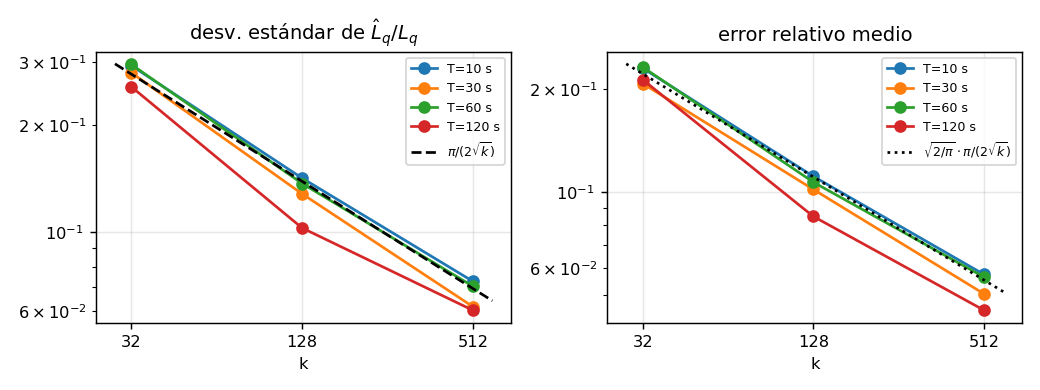
\includegraphics[width=\columnwidth]{act21_error_vs_k.png}
\caption{Desviación de $\Lh_q/L_q$ y error relativo medio contra $k$, por $T$ (5 semillas).}
\label{fig:errk}
\end{figure}

\begin{figure}[t]
\centering
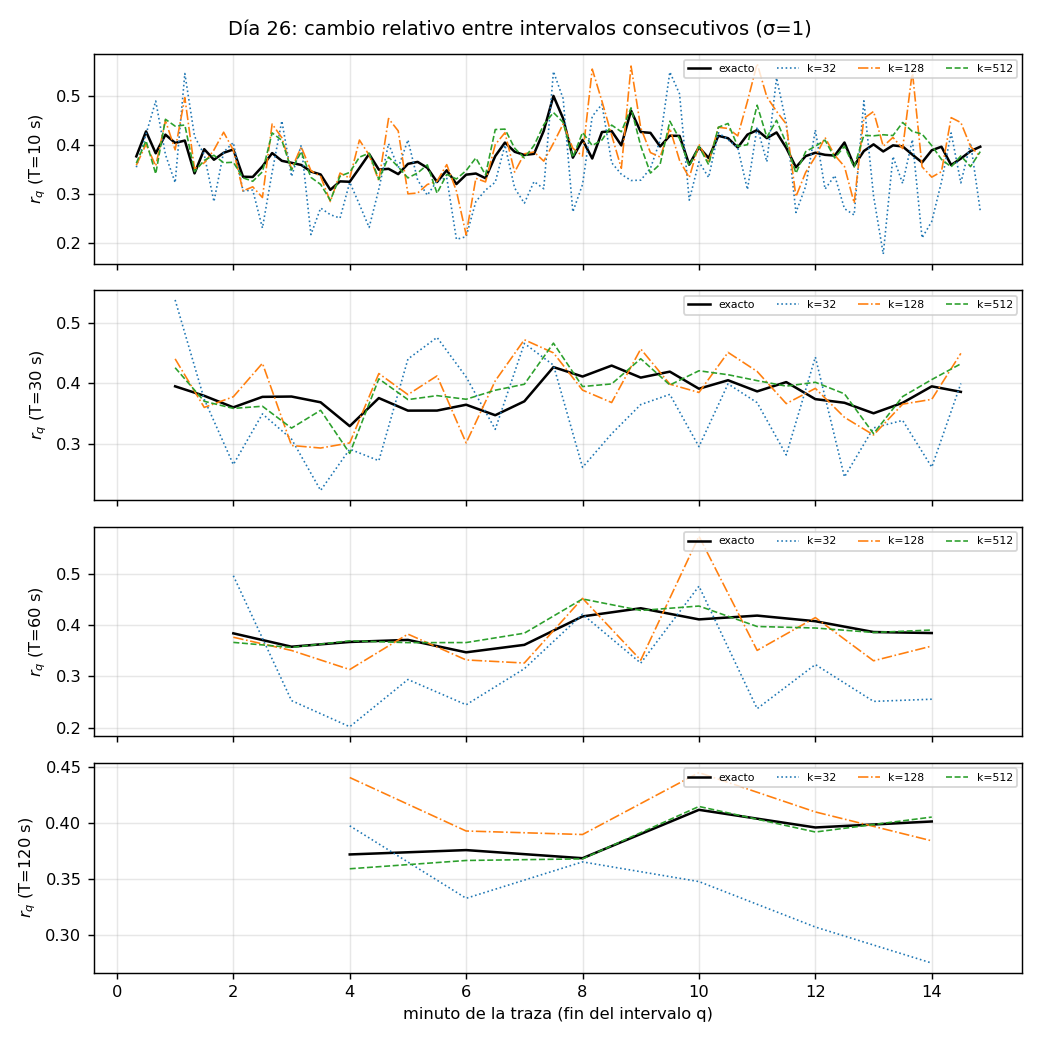
\includegraphics[width=\columnwidth]{act21_rq.png}
\caption{Día 26: $r_q$ exacto y estimado ($\sigma=1$), un panel por $T$.}
\label{fig:rq}
\end{figure}

\textbf{Caché} ($T=60$~s, $k=512$, traza precargada en RAM, ejecución en serie). La Tabla~\ref{tab:cache} muestra los resultados. La caché reduce las llamadas a \textsc{Actualizar} a $\phi_B=0{,}27$, $0{,}21$ y $0{,}19$, y multiplica el throughput por $2{,}3$--$3{,}6$. $\phi_B$ no baja de $\approx0{,}17$ porque esa es su cota inferior: cada IP distinta de cada intervalo cuesta al menos una llamada ($\sum_q|\mathrm{supp}(x_q)|/N=0{,}168$). La causa es que el 97,6\,\% de los 14,9~M destinos del día recibe \emph{un solo} paquete, casi todos ICMP de un mismo origen que barre el espacio de direcciones. Con $B=65536$ la caché ya está a 10\,\% de esa cota.

\begin{table}[t]
\centering
\caption{Efecto de la caché ($T=60$~s, $k=512$, día 26).}
\label{tab:cache}
\setlength{\tabcolsep}{4pt}
\begin{tabular}{lrrrr}
\toprule
$B$ & memoria & $\phi_B$ & tiempo & paquetes/s \\
\midrule
sin caché$^\dagger$ & 0 & 1,000 & 101,6~s & 68.089 \\
256 & 2~KiB & 0,267 & 646,3~s & 158.143 \\
4096 & 32~KiB & 0,210 & 428,8~s & 238.347 \\
65536 & 512~KiB & 0,186 & 421,4~s & 242.530 \\
\bottomrule
\multicolumn{5}{l}{\footnotesize $^\dagger$Solo el primer intervalo (6,92~M paquetes); el resto, la traza completa (102,2~M).}
\end{tabular}
\end{table}

\section{Comparación entre días (Actividad 2.2)}

\textbf{Días 25 y 26} ($\sigma=1$, $T=60$~s, 14 intervalos cerrados en ambas trazas). El sketch estima $\|x^{25}_q-x^{26}_q\|_1$ con un error medio de $3{,}8\,\%$ (p95 $7{,}9\,\%$) para $k=512$. Sumando los sketches de los 15 intervalos de cada día (incluido el último, vaciado), se obtiene $\Lh=207{,}2$~M frente a $L=205{,}68$~M exacto (error de $0{,}76\,\%$). Pero $r$ entre días vale $0{,}9999$ por minuto y $0{,}9989$ para la traza completa, frente a $r\approx0{,}39$ entre minutos consecutivos del mismo día (Fig.~\ref{fig:dias}). Es decir, los dos días casi no comparten IPs de destino, y $L\approx N^{25}+N^{26}$, mientras que $|N^{25}-N^{26}|=1{,}50$~M es 137 veces menor que $L$.

La causa no es el tráfico sino la \emph{anonimización}: MAWI anonimiza las direcciones con Crypto-PAn y \emph{``the mapping is consistent only within a single trace for daily traces''}~\cite{mawifaq}. Los datos lo confirman. La IP que más aporta a $L$ el día 25 (202.244.39.10: 23,3~M paquetes TCP, puertos de origen 443 (77\,\%) y 80 (20\,\%), 1.381~B de media, unos 5.500 orígenes) no aparece el día 26. En cambio, el día 26 aparece 202.83.161.53 con el mismo perfil (16,2~M paquetes, 443/80 en 78/20\,\%, 1.376~B, unos 4.900 orígenes): es el mismo servidor con otra etiqueta. Lo mismo ocurre con el destino ICMP con al menos $10^6$ orígenes (203.178.139.235 el día 25 y 203.76.138.16 el día 26). Comparar días con IPs anonimizadas mide cuánto cambia la etiqueta, no el tráfico.

\textbf{Semillas distintas.} Con $\sigma=1$ para el día 25 y $\sigma=2$ para el 26, el error entre días sigue siendo bajo ($4{,}5\,\%$, y $0{,}65\,\%$ en la traza completa), pero por casualidad. Con matrices distintas, $C_1a-C_2b$ tiene en cada fila la distribución de $(\|a\|_1+\|b\|_1)X$ (1-estabilidad aplicada a columnas independientes), y aquí $\|a-b\|_1\approx\|a\|_1+\|b\|_1$ porque los soportes son casi disjuntos. Para ver el efecto real se compararon minutos consecutivos del \emph{mismo} día con semillas distintas (minuto $q$ con $\sigma=1$ y minuto $q-1$ con $\sigma=2$): $\Lh/(N_q+N_{q-1})=0{,}98$ en promedio, es decir, $\Lh=2{,}54\,L$, frente a un error de $3{,}4\,\%$ con la misma semilla. Con semillas distintas, la parte compartida ya no se cancela y el sketch siempre responde ``todo cambió''.

\begin{figure}[t]
\centering
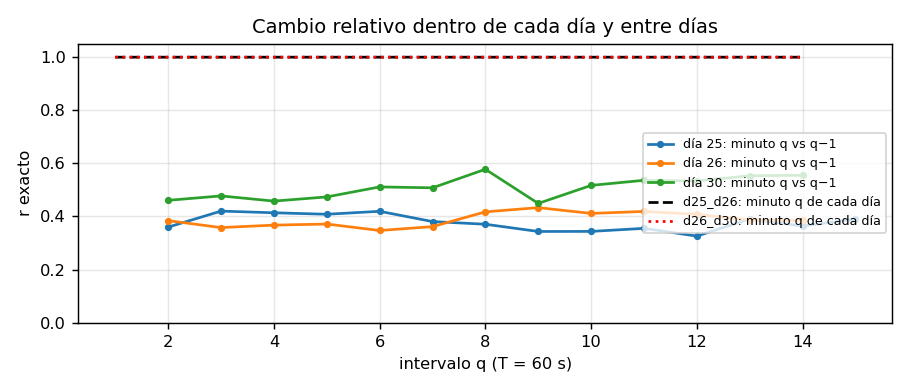
\includegraphics[width=\columnwidth]{act22_r_dias.png}
\caption{$r$ exacto entre minutos consecutivos de cada día y entre el mismo minuto de dos días ($T=60$~s).}
\label{fig:dias}
\end{figure}

\textbf{Contraste: días 26 y 30.} Entre días el resultado es igual, saturado por la anonimización: error $5{,}1\,\%$ por intervalo; $\Lh=193{,}6$~M frente a $L=195{,}0$~M (error de $0{,}71\,\%$); $r=0{,}9983$. Medido así, el cambio \emph{no} es mayor que entre los días 25 y 26: ambos están en $r\approx1$. Sí cambió, en cambio, el tráfico \emph{dentro} del día 30: el $r$ medio entre minutos consecutivos sube a $0{,}508$, frente a $0{,}377$ y $0{,}388$ los días 25 y 26 (Fig.~\ref{fig:dias}). Como las IPs no se pueden emparejar entre días, el tráfico se caracterizó por su perfil (\texttt{bin/perfil}, Tabla~\ref{tab:perfil}):

\begin{table}[t]
\centering
\caption{Perfil de cada traza. ``1~pkt'': destinos que reciben un solo paquete en los 15 minutos.}
\label{tab:perfil}
\setlength{\tabcolsep}{3pt}
\begin{tabular}{lrrr}
\toprule
 & día 25 & día 26 & día 30 \\
\midrule
paquetes IPv4 & 103,7~M & 102,2~M & 93,2~M \\
TCP / UDP / ICMP (\%) & 69,8/8,7/19,6 & 69,2/9,0/19,7 & 57,7/17,1/22,8 \\
destinos distintos & 14,80~M & 14,89~M & 21,71~M \\
destinos de 1~pkt & 14,45~M & 14,54~M & 21,26~M \\
\quad de ellos ICMP & 14,43~M & 14,51~M & 14,65~M \\
\quad de ellos UDP/53 & 902 & 791 & 6,58~M \\
UDP/53 sobre UDP & 1,5\,\% & 1,6\,\% & 43,0\,\% \\
\bottomrule
\end{tabular}
\end{table}

\begin{itemize}
\item \textbf{Escaneo DNS nuevo.} Un solo origen (anonimizado como 203.90.255.0) envía UDP al puerto 53 a \textbf{6,58~M destinos distintos, un paquete a cada uno}. UDP pasa de 9,0\,\% a 17,1\,\% del tráfico, el puerto 53 pasa de 1,6\,\% a 43\,\% del UDP, y los destinos distintos suben de 14,9~M a 21,7~M. Cada paquete de un escaneo va a un destino nuevo y aporta 1 a $L$ en cada minuto, lo que explica el alza de $r$ dentro del día.
\item \textbf{El barrido ICMP es estable.} Los tres días, un origen envía ICMP a $\approx$14,5~M destinos (un paquete cada uno) y recibe respuestas de al menos $10^6$ orígenes. En el día 30, ese destino ICMP (203.90.235.204, 5,6~M paquetes) es el tercero que más aporta a $L$. Es tráfico habitual, no la novedad.
\item \textbf{Menos TCP masivo.} TCP baja de 70,8~M a 53,8~M paquetes. El mayor destino HTTPS del día 26 (16,2~M paquetes, 8,3\,\% de $L_{26,30}$) no tiene equivalente de ese tamaño el día 30, donde el mayor destino TCP tiene 7,3~M.
\end{itemize}
Las 10 IPs que más aportan explican el 27,8\,\% de $L_{26,30}$ (34,8\,\% de $L_{25,26}$). Son los grandes servidores HTTPS y los destinos ICMP de cada día, cada uno presente solo en su propia traza.

\section{Preguntas}

\textbf{1. 1-estabilidad y mediana.} Por linealidad, $y^a-y^b=C(a-b)$, y por 1-estabilidad cada fila es $\|a-b\|_1X_j$ con $X_j$ Cauchy: es una medición de $L$ multiplicada por un factor aleatorio. Como $P(|X|\le1)=\frac2\pi\arctan1=\frac12$, la mediana de $|X_j|$ es 1 y la mediana muestral de $|y^a_j-y^b_j|$ converge a $L$, con un error de $\pi/(2\sqrt k)$. El promedio no sirve porque $E|X|=\infty$: no converge, y unas pocas filas enormes lo dominan. La cola $P(|X|>t)\approx2/(\pi t)$ se cumple en nuestros pesos: el cuantil 0,999 de $|C|$ vale 650.

\textbf{2. Error observado.} Coincide con la teoría: la desviación de $\Lh/L$ es $0{,}26$--$0{,}30$, $0{,}10$--$0{,}14$ y $0{,}060$--$0{,}073$ frente a $0{,}278$, $0{,}139$ y $0{,}069$, y no depende de $T$, aunque $L_q$ varía en un factor 10. En la Tarea~1, en cambio, el error de CMS escalaba como $\|f\|_1/w$ y el de CountSketch como $\|f\|_2/\sqrt w$: dependía del volumen del tráfico y de las colisiones. Allí, para una IP grande se obtenían errores relativos de $0{,}01$--$4\,\%$ con decenas de KiB a 1~MiB, porque esa IP dominaba la norma. Aquí el error relativo está fijado solo por $k$ (7\,\% con 4~KiB por sketch), aunque se estima una cantidad global sobre millones de IPs. La garantía es multiplicativa y no depende del tráfico, pero para bajar al 1\,\% hacen falta $k\approx25.000$ filas.

\textbf{3. Misma semilla.} La resta solo cancela el tráfico compartido si cada IP usa la misma columna $C_{\cdot,i}$ en ambos sketches. Con semillas distintas, $C_1a-C_2b$ estima $\|a\|_1+\|b\|_1$ y no $\|a-b\|_1$. Lo medimos en minutos consecutivos del día 26: $\Lh=0{,}98(N_q+N_{q-1})=2{,}54\,L$. Con la misma $\sigma$, dos routers comparten la matriz sin transmitirla y basta enviar $k$ números.

\textbf{4. $\|a-b\|_1$ frente a $|N_a-N_b|$.} $|N_a-N_b|$ solo detecta cambios de volumen. Entre minutos consecutivos del día 26, $L_q\approx5$~M mientras que $|N_q-N_{q-1}|$ va de 0,06 a 0,58~M: la mayor parte del cambio redistribuye tráfico entre IPs sin alterar el total. Entre días, $|N^{25}-N^{26}|=1{,}5$~M y $L=205{,}7$~M. Ejemplo de un cambio que $|N_a-N_b|$ no detecta: un DDoS que desvía 1~M paquetes por minuto de un servidor legítimo hacia una víctima, o un escaneo como el del día 30 que coincida con una caída equivalente del tráfico normal. En ambos casos $N$ no cambia, pero $L$ crece en 2~M.

\section{Conclusiones}
El sketch de Cauchy implementado reproduce los valores de referencia y cumple la teoría: su error relativo es $\approx\pi/(2\sqrt k)$ (7\,\% con $k=512$), no depende de $T$ ni del volumen, y usa 40~KiB frente a los 20--179~MiB de la tabla exacta. La caché de mapeo directo es exacta y reduce las llamadas a \textsc{Actualizar} al 19--27\,\% (hasta 3,6 veces más throughput), cerca de la cota que impone el escaneo ICMP de un paquete por destino. Gracias a la linealidad, la suma de sketches estima el cambio entre trazas completas con un error menor a 1\,\%. Pero entre días $r\approx1$ por la anonimización por traza de MAWI: la métrica es correcta, mientras que los identificadores no son comparables entre días. El día 30 se distingue dentro de su propia traza ($r$ consecutivo 0,51 frente a 0,38) por un escaneo DNS a 6,6~M destinos que duplica la fracción UDP.

\begin{thebibliography}{1}
\bibitem{indyk} P.~Indyk, ``Stable distributions, pseudorandom generators, embeddings, and data stream computation,'' \emph{J. ACM}, 53(3), 2006 (versión FOCS 2000).
\bibitem{mawifaq} MAWI Working Group, ``MAWI Traffic Archive FAQ,'' \url{https://mawi.wide.ad.jp/mawi/faq.html}.
\bibitem{mawi} MAWI Working Group Traffic Archive, samplepoint-F, 2018, \url{https://mawi.wide.ad.jp/mawi/samplepoint-F/2018/}.
\end{thebibliography}

\end{document}
